\documentclass{article}
\usepackage{tikz}
\usepackage{pgfplots}
\pgfplotsset{width=7cm,compat=1.8}
\usepackage{pgfplotstable}
\usepackage{adjustbox}
\usepackage{diagbox}
\usepackage{colortbl}
\definecolor{LightRed}{RGB}{252,160,140}
\definecolor{LightBlue}{RGB}{140,186,252}
\newcolumntype{a}{>{\columncolor{LightRed}}c}

\begin{document}


%\diagbox[width=0.6 \textwidth/2, height=1cm]{Disciplinas}{Fases} & Inicio
%Elaboraci\'on & Construcci\'on & Transici\'on
    
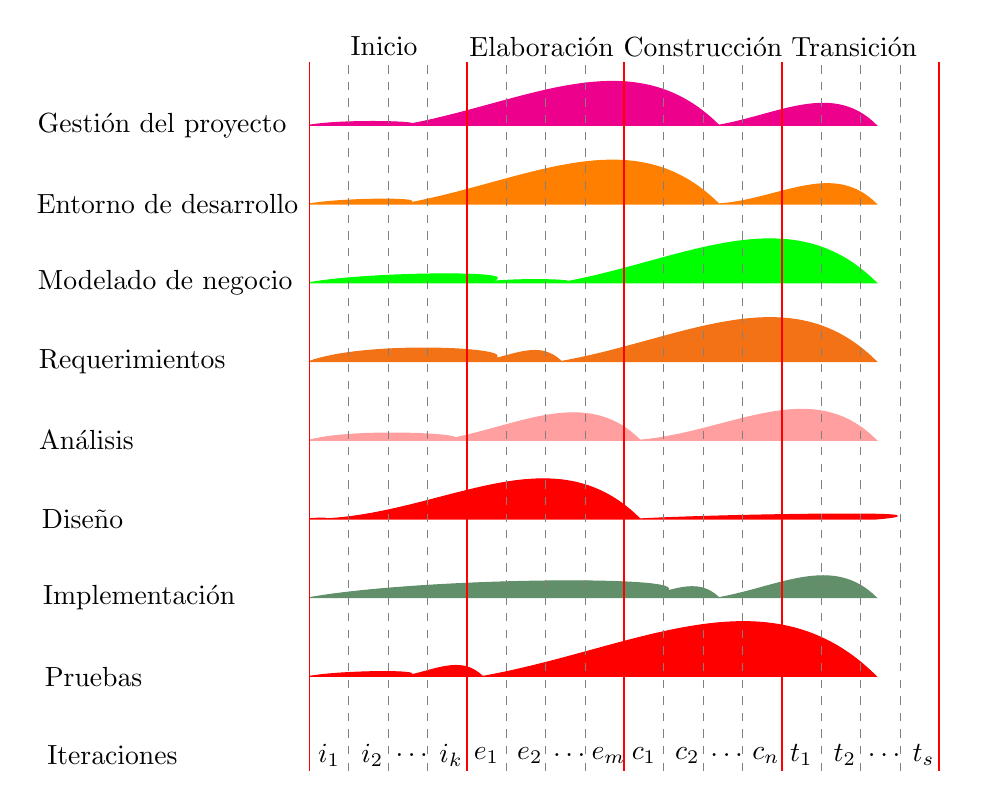
\begin{tikzpicture} 
\node[] (f1) at (5.75,3) {Inicio}; 
\node (f2) at (7.75,3) {Elaboraci\'on};
\node (f3) at (9.8,3) {Construcci\'on};
\node (f4) at (11.72,3) {Transici\'on};

\node (d1) at (2.93,2) {Gesti\'on del proyecto}; 
\draw[fill,color=magenta] (4.8,2) to[out=10, in=5] (6,2) to[out=10] (10,2) to[out=10] (12,2) to (4.8,2);
\node (d2) at (3,1) {Entorno de desarrollo};
\draw[fill,color=orange] (4.8,1) to[out=10, in=10] (6,1) to[out=10] (10,1) to[out=4] (12,1) to (4.8,1);
\node (d3) at (2.97,0) {Modelado de negocio};
\draw[fill,color=green] (4.8,0) to[out=10, in=10] (7,0) to[out=10,in=5] (8,0) to[out=10] (12,0) to (4.8,0);
\node (d4) at (2.55,-1) {Requerimientos};
\draw[fill,color=yellow!40!red] (4.8,-1) to[out=20, in=10] (7,-1) to[out=10] (8,-1) to[out=10] (12,-1) to (4.8,-1);
\node (d5) at (1.97,-2) {Análisis};
\draw[fill,color=pink!150] (4.8,-2) to[out=15, in=5] (6.5,-2) to[out=10] (9,-2) to[out=5] (12,-2) to (4.8,-2);
\node (d6) at (1.92,-3) {Dise\~no};
\draw[fill,color=red!100!yellow] (4.8,-3) to[out=10,in=10] (5,-3) to[out=3] (9,-3) to[out=3,in=5] (12,-3) to (4.8,-3);
\node (d7) at (2.64,-4) {Implementaci\'on};
\draw[fill,color=magenta!34!green] (4.8,-4) to[out=10, in=10] (9,-4) to[out=10] (10,-4) to[out=10] (12,-4) to (4.8,-4);
\node (d8) at (2.06,-5) {Pruebas};
\draw[fill,color=red] (4.8,-5) to[out=10, in=10] (6,-5) to[out=10] (7,-5) to[out=10] (12,-5) to (4.8,-5);

\node (i) at (2.3,-6) {Iteraciones};
\draw[help lines,color=orange!270,line width=0.02cm] (4.8,-6.2) -- (4.8,2.8);
\node (i1) at (5.05,-6) {$i_1$};
\draw[help lines,dashed] (5.3,-6.2) -- (5.3,2.8);
\node (i2) at (5.6,-6) {$i_2$};
\draw[help lines,dashed] (5.8,-6.2) -- (5.8,2.8);
\node (i3) at (6.1,-6) {$\ldots$};
\draw[help lines,dashed] (6.3,-6.2) -- (6.3,2.8);
\node (i3) at (6.6,-6) {$i_k$};

\draw[help lines,color=orange!270,line width=0.02cm] (6.8,-6.2) -- (6.8,2.8);
\node (i1) at (7.05,-6) {$e_1$};
\draw[help lines,dashed] (7.3,-6.2) -- (7.3,2.8);
\node (i2) at (7.6,-6) {$e_2$};
\draw[help lines,dashed] (7.8,-6.2) -- (7.8,2.8);
\node (i3) at (8.1,-6) {$\ldots$};
\draw[help lines,dashed] (8.3,-6.2) -- (8.3,2.8);
\node (i3) at (8.6,-6) {$e_m$};

\draw[help lines,color=orange!270,line width=0.02cm] (8.8,-6.2) -- (8.8,2.8);
\node (i1) at (9.05,-6) {$c_1$};
\draw[help lines,dashed] (9.3,-6.2) -- (9.3,2.8);
\node (i2) at (9.6,-6) {$c_2$};
\draw[help lines,dashed] (9.8,-6.2) -- (9.8,2.8);
\node (i3) at (10.1,-6) {$\ldots$};
\draw[help lines,dashed] (10.3,-6.2) -- (10.3,2.8);
\node (i3) at (10.6,-6) {$c_n$};

\draw[help lines,color=orange!270,line width=0.02cm] (10.8,-6.2) -- (10.8,2.8);
\node (i1) at (11.05,-6) {$t_1$};
\draw[help lines,dashed] (11.3,-6.2) -- (11.3,2.8);
\node (i2) at (11.6,-6) {$t_2$};
\draw[help lines,dashed] (11.8,-6.2) -- (11.8,2.8);
\node (i3) at (12.1,-6) {$\ldots$};
\draw[help lines,dashed] (12.3,-6.2) -- (12.3,2.8);
\node (i3) at (12.6,-6) {$t_s$};
\draw[help lines,color=orange!270,line width=0.02cm] (12.8,-6.2) -- (12.8,2.8);

%\draw[fill,color=softgreen] (10,-6) to[out=10, in=10] (13,-6) to[out=10] (16,-6) to[out=10] (18,-6) to (10,-6);
\end{tikzpicture}

\end{document}